\chapter{Spatial Domain: \refmod}
\label{ch:ref-mod}

It was Xenakis' goal for the curved surfaces of the Philips Pavilion
to reduce the sonic contribution of sound
reflections.\cite{philips1958} He knew that reflections and the
resulting comb filtering could impair intelligibility and localization
of music and sounds.  The pavilion was to have hundreds of
loudspeakers, and an elaborate custom sequencer was selecting which
speakers Edgard Var\`{e}se music played from. The acoustics of the
space was certainly an important concern during the design process:
Xenakis wanted to compose the space as he would a piece of music.
Today we have a better understanding of indoor acoustics and sound
reinforcement, and some of Xenakis' motivations seem
questionable. Large curved surfaces are more likely to cause
temporally diffuse acoustic reflections, while Large flat surfaces
will cause specular (non-diffuse) reflections. There is evidence that
curved surfaces such as stage shells can be quite effective for the
performers of acoustic music.\cite{DAntonio1991} However, in the
context of loudspeaker playback, the advantages of curved surfaces
over flat (non-parallel) surfaces are somewhat ambiguous.\cite{Cox2006}

\section{Composing with Space}
\label{sec:composing-with-space}
If Xenakis had been able to 

\begin{figure*}[]
  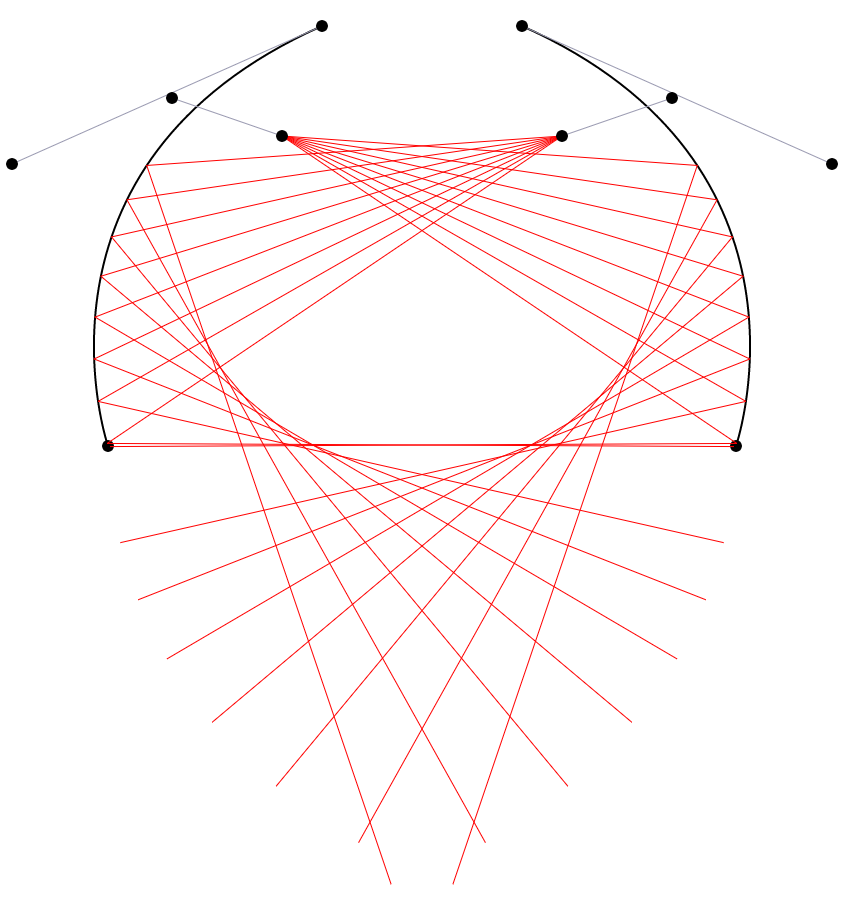
\includegraphics[width=\linewidth]{refmod/refmod.png}
  \caption[Tempo Transition]{\refmod user interface.}
  \label{fig:basic-tempo-change}
\end{figure*}


%%% Local Variables:
%%% mode: latex
%%% TeX-master: "CharlesHolbrow_MAS_Thesis"
%%% End:
